%
% File naaclhlt2018.tex
%
%% Based on the style files for NAACL-HLT 2018, which were
%% Based on the style files for ACL-2015, with some improvements
%%  taken from the NAACL-2016 style
%% Based on the style files for ACL-2014, which were, in turn,
%% based on ACL-2013, ACL-2012, ACL-2011, ACL-2010, ACL-IJCNLP-2009,
%% EACL-2009, IJCNLP-2008...
%% Based on the style files for EACL 2006 by 
%%e.agirre@ehu.es or Sergi.Balari@uab.es
%% and that of ACL 08 by Joakim Nivre and Noah Smith

\documentclass[11pt,a4paper]{article}
\usepackage[hyperref]{naaclhlt2018}
\usepackage{times}
\usepackage{latexsym}
\usepackage{graphicx}
\usepackage{soul}
\usepackage{color}

\usepackage{url}

\aclfinalcopy % Uncomment this line for the final submission
%\def\aclpaperid{***} %  Enter the acl Paper ID here

%\setlength\titlebox{5cm}
% You can expand the titlebox if you need extra space
% to show all the authors. Please do not make the titlebox
% smaller than 5cm (the original size); we will check this
% in the camera-ready version and ask you to change it back.

\hypersetup{draft}
\newcommand\BibTeX{B{\sc ib}\TeX}

\title{Modeling Second-Language Learning from a Psychological Perspective}


\author{Alexander S. Rich\qquad Pamela J. Osborn Popp\qquad David J. Halpern\\
  \textbf{Anselm Rothe\qquad Todd M. Gureckis} \\
  Department of Psychology, New York University \\
  {\tt \{asr443,pamop,david.halpern,anselm,todd.gureckis\}@nyu.edu} \\}

\date{}

\begin{document}
\maketitle
\begin{abstract}
Psychological research on learning and memory
has tended to emphasize small-scale laboratory
studies.  However, large datasets of people using 
educational software provide opportunities to explore
these issues from a new perspective.  In this paper we
describe our approach to the Duolingo Second Language
Acquisition Modeling (SLAM) competition which was run in
early 2018.  We used a well-known class of algorithms (gradient boosted decision
trees), with features partially informed by theories from the psychological
literature. After detailing our modeling approach and a number of
supplementary simulations, we
reflect on the degree to which psychological theory aided the model, and
the potential for cognitive science and predictive modeling competitions to gain
from each other.
\end{abstract}

\section{Introduction}

Educational software that aims to teach people new skills, languages, and
academic subjects have become increasingly popular.  The wide-spread
deployment of these tools has created interesting opportunities to study
the process of language acquisition in extremely large samples of learners in naturalistic
situations. The Duolingo shared task on Second Lanugage Acquisition Modeling (SLAM)
was a competitive modeling challenge run in early 2018~\cite{slam18}.
The challenge, organized by Duolingo\footnote{http://duolingo.com}, a popular second
language learning app, was
to use log data from thousands of users completing millions of exercises to 
predict patterns of future translation mistakes in held-out data.  The data was
divided into three sets covering Spanish speakers learning English ({\tt en\_es}),
English speakers learning Spanish ({\tt es\_en}), and English speakers learning
French ({\tt fr\_en}).
This paper reports the approach used by our team which ended in third place 
for the {\tt en\_es} data set, second place for {\tt es\_en}, and third place
for {\tt fr\_en}.



Learning and memory has been a core focus of psychological science for
over 100 years. Most of this work has sought to build explanatory theories of human learning
and memory using relatively small-scale laboratory studies.  Such studies have
identified a number of important and apparently robust phenomena in memory including
the nature of the retention curve~\cite{Rubin:1996aa}, the advantage for spaced over massed 
practice~\cite{Ruth:1928aa,Cepeda:2006aa,Mozer:2009cs}, the testing effect~\cite{Roediger2006te},
and retrieval-induced forgetting~\cite{Anderson1994rif}.
The advent of large datasets such as the one provided in the Duolingo SLAM challenge
may offer a new perspective and approach which may prove complementary
to laboratory scale science~\cite{Griffiths:2015aa,Goldstone:2016aa}.  First, the much
larger sample sizes may help to better identify parameters of psychological models.
Second, datasets covering more naturalistic learning situations may allow us to test 
the predictive accuracy of psychological theories in a more generalizable fashion~\cite{Yarkoni:2017aa}.

Despite these promising opportunities, it remains unclear how much of current psychological
theory might be important for tasks such as the Duolingo SLAM challenge.
As one example, the field of education data mining which has attempted to build
predictive models of student learning have found excellent results using
deep neural networks~\cite[so called ``deep knowledge tracing",][]{Piech:2015aa} 
as opposed to more traditional, and interpretable, models and approaches
that are rooted in cognitive science~\cite[e.g.,][]{Atkinson:1972rm,Atkinson:1972rz,Corbett1995bkt,Pavlik:2008rm,Tubridy:2018ab}. 
Recently, Khajah, Lindsey, \& Mozer (2016) compared deep knowledge tracing (DKT) to a more
standard ``Bayesian knowledge tracing" (BKT) models and showed
that it was possible to equate the performance of the the BKT model by additional 
features and parameters that represent core aspects of the psychology of learning
and memory such as forgetting~\cite{Khajah2016hdnt}.

Our entry to SLAM borrowed conceptually from the Khajah et al. (2016) approach.
Specifically we used a relatively well known and powerful classification
algorithm: gradient boosting decision trees~\cite[GBDT][]{ke2017lightgbm}.  Like
deep learning, this algorithm can extract complex interactions among features,
but it has some advantages including faster training and easier integration of
diverse inputs. We then created a number of new features for the SLAM
dataset covering aspect such as user perseverance, learning processes, 
contextual factors, and cognate similarity.  After finding a model which provided the best
held-out performance on the test data set, we conducted a number of ``lesioning" studies where
we selectively removed features from the model and re-estimated the parameters in order
to assess the contribution of particular types of features.  We being by describing our 
overall modeling approach, and then discuss some of the lessons learned from our analysis.


\section{Task Approach}

We approached the task as a binary classification problem over instances (i.e.,
single words within an exercise). Our solution can be divided into two
components---constructing a set of features that is highly informative about
whether the user will answer an instance correctly, and designing a model that
can achieve high performance using this feature set.

\subsection{Feature Engineering}

We used a variety of features, including features directly present in the
training data, features constructed using the training data, and features that
use information external to the training data. Except where otherwise specified,
categorical variables were one-hot encoded.

\subsubsection{Exercise features}

We encoded the exercise number, client, session, format, and duration (i.e., number of
seconds to complete the exercise), as well as the time since the user started using Duolingo for the first time.

\subsubsection{Word features}

Using spaCy\footnote{https://spacy.io/}, we lemmatized each word to produce a root word. Both the root
word token and the original token were used as categorical features. Due to
their high cardinality, these features were not one-hot encoded but were
preserved in single columns and handled in this form by the model (as described
below).

Along with the tokens themselves we encoded each instance word's part of speech,
morphological features, and dependency edge label. (We noticed that some words
in the original dataset were paired with the wrong morphological features,
particularly near where punctuation had been removed from the sentence. To fix
this, we re-processed the data using Google SyntaxNet\footnote{https://github.com/ljm625/syntaxnet-rest-api}.)

We also encoded word length and several word characteristics gleaned from
external data sources. Past research suggests that uncommon words are harder to process than common words; readers will look longer at low-frequency words and perform worse in word-identification tasks for these than for high-frequency words \cite{rayner1998eye}. We therefore included a feature that encoded the frequency of each word in the language being acquired, calculated from \citet{robert_speer_2017_998161}. A number of studies have also shown that age-of-acquisition (i.e., the age a which children typically exhibit this word in their vocabulary) is another strong predictor of word processing and lexical retrieval difficulty that is somewhat independent of word frequency \cite{brysbaert2011effects, ferrand2011comparing}. We therefore included mean age-of-acquisition (in English) as a feature, derived from published age-of-acquisition norms for 30,000 English words from \cite{Kuperman2012} which covered many of the words present in the dataset. Additionally, cognates, or words sharing a common linguistic derivation, are easier to learn than words with dissimilar translations \cite{de2000hard}. As an approximate measure of linguistic similarity, we used the Levenshtein edit distance between the word tokens and their translations scaled by the length of the longer word. We found translations using Google Translate\footnote{https://cloud.google.com/translate/} and calculated the Levenshtein distance to reflect the letter-by-letter similarity of the word and its translation \cite{hyyro2001explaining}. 

\subsubsection{User features}

Just as we did for word tokens, we encoded the user ID as a single-column,
high-cardinality feature. We also calculated several other user-level features that related to the ``learning type'' of a user. In particular, we encoded features to estimate the long-term motivation and diligence of a user. These features could help predict how users interact with old and novel words they encounter.

%Feature 1: Motivation %compute_motivation
To estimate users' motivation we grouped their exercises into ``bursts.'' Bursts
were separated by at least 24 hours \hl{todd says: did you change my code
  because bursts were separate by 1 hour in my imementation}.  We used three
concrete features about these bursts, namely the mean and median number of
exercises within bursts as well as the total number of bursts of a given user.
We hypothesized that more motivated users may have bursts with more exercises.
Simultaneously, a larger total number of bursts indicated that the burst length
estimate was more trustworthy.

%Feature 2: Consistency %compute_usage_entropy

To estimate users' diligence we speculated that a very diligent user might be using the app regularly at the same time of day, perhaps following a study schedule, compared to a less diligent user whose schedule might vary more. The data set did not provide a variable with the time of day, which would have been an interesting feature on its own. Instead, we were able to extract for each exercise the time of day relative to the first time a user had used the app, ranging from 0 to 1 (with 0 indicating the same time, 0.25 indicating a relative shift by 6 hours, etc.).  We then discretized this variable into 20-minute bins and computed the entropy of the empirical frequency distribution over these bins. A lower entropy score indicated less variability in the times of day a user started their exercises.

\subsubsection{Positional features}

To account for the effects of surrounding words on the difficulty of an
instance, we created several features related to the instance word's context in
the exercise. These included the token of the previous word, the next word, and
the instance word's root in the dependency tree, all stored in single columns as with
the instance token itself. We also included the part of speech of each of these
context words as additional features. When there was no previous word, next word, or dependency-tree
root word, a special {\tt None} token or {\tt None} part of speech was used.

\subsubsection{Temporal features}

A user's probability of succeeding on an instance is likely related to their
prior experience with that instance. To capture this, we calculated several
features related to past experience. 

First, we encoded the number of times the
current exercise's exact sentence had been seen before by the user. This is
informed by psychological research showing memory and perceptual processing
improvement for repeated contexts or chunks~\cite[e.g.,][]{Chun:1999gt} 

We also encoded a set of features recording past experience with
the particular instance word. These features were encoded separately for the
instance token and for the instance root word created by lemmatization.
For each token (and root) we tracked user performance through four weighted
error averages. At the user's first encounter of the token, each error term $E$ starts at
zero. After an encounter with an instance of the token with label $L$ (0 for
success, 1 for error), it is
updated according to the equation

\[
E \leftarrow E + \alpha (L - E)
\]

where $\alpha$ determines the speed of error updating. The four weighted
error terms use $\alpha = \{.3, .1, .03, .01\}$, allowing both short-run and
long-run changes in a user's error rate with a token to be tracked. Note that in
cases where a token appears multiple times in an exercise, a single update of
the error features is conducted using the mean of the token labels.
Along with the error tracking features, for each token we calculated the number
of labeled, unlabeled, and total encounters; time since last labeled encounter and
last encounter; and whether the instance is the first encounter with the
token.

In the training data, all instances are labeled as correct or incorrect, so the
label for the previous encounter is always available. In the test data, labels
are unavailable, so predictions must be made using a mix of labeled and
unlabeled past encounters. To generate training-set features that are 
comparable to test-set features, we selectively ignored some labels when encoding temporal features on
the training set. Specifically, for each user we first calculated the number of
exercises $n$ in the true test set. Then, when encoding the features for each
instance, we selected a random integer $r$ in the range $[1,n]$, and ignored labels
in the prior $r$ exercises. That is, we encode features for the current instance
as though other instances in those prior exercises were unlabeled, and ignore
updates to the error averages from those exercises. The result of this process
is that each instance in the training set is encoded as though it were between
one and $n$ exercises into the test set.

\subsection{Modeling}

\begin{table}[t!]
\small
\begin{center}
\begin{tabular}{|l|llll|}
  % \hline   & \multicolumn{3}{l}{\bf Value} & \\
  \hline \bf Parameter & {\tt fr\_en} & {\tt en\_es} & {\tt es\_en} & {\tt all} \\ \hline
  num\_leaves & 256 & 512 & 512 & 1024 \\
  learning\_rate & .05 & .05 & .05 & .05 \\
  min\_data\_in\_leaf & 100 & 100 & 100 & 100 \\
  num\_boost\_rounds & 750 & 650 & 600 & 750 \\
  cat\_smooth & 200 & 200 & 200& 200 \\
  feature\_fraction & .7 & .7 & .7 & .7 \\
  max\_cat\_threshold & 32 & 32 & 32& 64 \\
\hline
\end{tabular}
\end{center}
\caption{\label{lightgbm-params} Parameters of final LightGBM models. See
  LightGBM documentation for more information; all other parameters were left at
their default values.}
\end{table}

After featurizing the training data, we trained GBDT models to minimize log loss. GBDT works by
iteratively building regression trees, each of which seeks to minimize the
residual loss from prior trees. This allows it to capture non-linear effects
and high-order interactions among features. We used the LightGBM\footnote{http://lightgbm.readthedocs.io/} implementation
of GBDT \cite{ke2017lightgbm}.

For continuous-valued features, GBDT can split a leaf at any point, creating
different predicted values above and below that threshold. For categories that
are one-hot encoded, it can split a leaf on any of the category's features. This
means that for a category with thousands of values, potentially thousands of
tree splits would be needed to capture its relation to the target. Fortunately,
LightGBM implements an algorithm for partitioning the values of a categorical
feature into two groups based on their relevence to the current loss, and create
a single split to divide those groups \cite{fisher1958grouping}. Thus, as
alluded to above, high-cardinality features like token and user ID were encoded as
single columns and handled as categories by LightGBM.

We trained a model for each of the three language tracks of {\tt en\_es}, {\tt es\_en},
and {\tt fr\_en}, and also trained a model on the combined data from
all three tracks, adding an additional ``language'' feature. Following model
training, we averaged the predictions of each single-language model with that of
the all-language model to form our final predictions.

To tune model hyper-parameters and evaluate the usefulness of features, we first
trained the models on the {\tt train} data set and evaluated them on the {\tt dev}
data set. Once the model structure was finalized, we trained on the combined
{\tt train} and {\tt dev} data and produced predictions for the {\tt test} data. The
LightGBM hyperparameters used for each model are listed in Table~\ref{lightgbm-params}.



\subsection{Performance}

The AUROC of our final predictions was $.8585$ on {\tt en\_es}, $.8350$ on {\tt
  es\_en}, and $.8540$ on {\tt fr\_en}. We did not attempt to optimize the model's
F1 score, but the F1 score could likely be improved (at the cost of
increased log loss) by finding the
rescaling of the {\tt dev} predicted probabilities that maximized the F1 score at
the 0.5 threshold, and applying this rescaling to the {\tt test} predicted probabilities.

\section{Feature Removal Experiments}

\begin{figure*}[htp]
% \centering
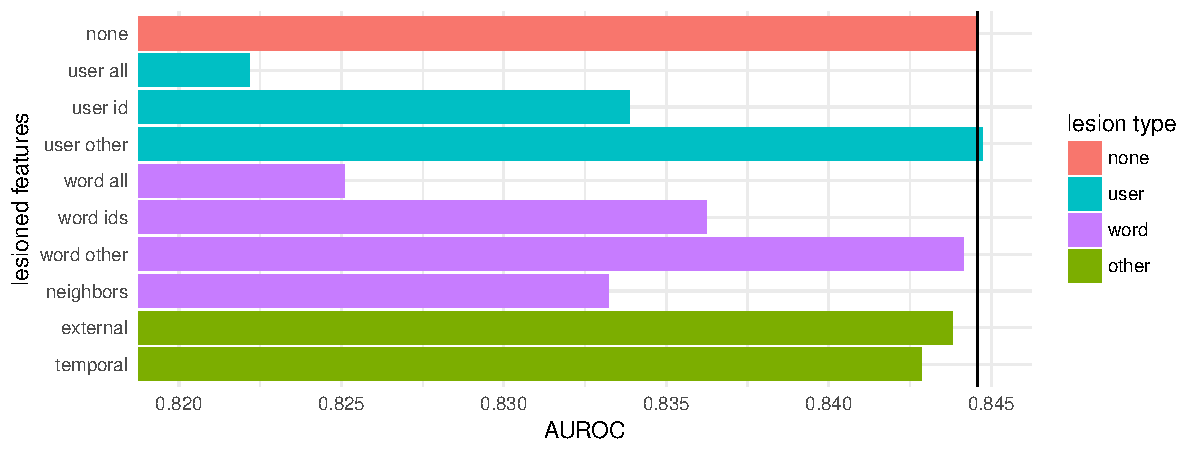
\includegraphics[width=\textwidth]{lesions.pdf}
\caption{Performance on {\tt dev} of models trained on all {\tt train} data,
  with different groups of lesioned features. See main text for description of
  lesion groups}
\label{fig:lesions}
\end{figure*}


To better understand which features or groups of features were most important to
our model's predictions, we conducted a set of experiments in which we lesioned
(i.e., removed) a group of features and re-trained the model on the {\tt train}
set, evaluating performance on the {\tt dev} set. For simplicity, we ran each of the
lesioned models on all language data and report the average
performance. We did not run individual-language models as we did for our primary model.

The results of the lesion experiments are shown in Figure~\ref{fig:lesions}. The
models are as follows.
\begin{description}
  \item[none:] all features are included.  
  \item[user:] all user-level features, including the user ID and other
    calculated features like entropy and measures of exercise bursts, are
    removed.
  \item[userid \& user other:] only user ID or only the calculated
    features user features, respectively, are removed.
  \item[word:] Token and token root IDs; previous, next, and dependency-tree
    root word IDs; and morphological, part of speech, and dependency tree
    features are removed.
  \item[word id \& word other:] only word IDs or only other
    word features, respectively, are removed.
  \item[neighbors:] Both word IDs and other word features are removed, but
    only for the previous, next, and dependency-tree root words. Information
    about the present word is maintained.
  \item[external:] External information about the word, including corpus
    frequency, Levenshtein distance from translation, and age of acquisition,
    are removed.
  \item[temporal:] Temporal information, including number and timing of
    past encounters with the word and error tracking information, is removed.
\end{description}

Interestingly, we found that for both user-level and word-level features, the
bulk of the model's predictive power could be achieved using ID's alone,
represented as high-cardinality categorical features. Removing other word features,
such as morphological features and part of speech, created only a small
degradation of performance. In the case of users, removing features such as
entropy and average exercise burst length led to a tiny increase of performance.
In the case of both users and words, though, we find that in the absence of ID
features the other features are helpful and lead to better performance than
removing all features. We also found that removing all information about
neighboring words and the dependency-parse root word degraded performance. This
confirms that word context matters, and suggests that users commonly make errors in word order,
subject--verb matching and other grammatical rules.

Our external word features---Levenshtein distance to translation, frequency, and
age of acquisition---provided a slight boost to model performance, showing the
benefit of considering what makes a word hard to learn from a psychological and
linguistic perspective. Adding temporal features about past encounters and
errors helped the models, but not as much as we expected. While not included in
the final model, we had also tried augmenting the temporal feature set with more
features related to massing and spacing of encounters with a word, but found it
did not improve performance. This is perhaps not surprising given how small the
benefit of the existing temporal features are in our model.

Though not plotted above, we also ran a model lesioning exercise-level features
including client, session type, format, and exercise duration. This model
achieved an AUROC of $.787$, far lower than any other lesion. This points to the
importance of how a question is asked for user performance, reflecting insights
from psychology such as the difference between recall and recognition memory
\cite{yonelinas2002nature}.

\section{Discussion}

When approaching the Duolingo SLAM task, we hoped to leverage psychological
insights in building our model. We found that in some cases, such as using the
word's age of acquisition, this was helpful. In general, though, our model gained its
power not from hand-crafted features but from applying a powerful inference
technique (gradient boosted decision trees) to raw input about user and word IDs and
exercise features.

There are multiple reasons for the limited applicability of psychology to this
competition. First, computational psychological models, while useful, are not
well-suited to generating highly accurate predictions from large data sets.
Because they are designed not for prediction but for explanation, they tend to
use a small number of input variables and allow those variables to interact
in limited ways. In contrast, gradient boosted decision trees, as well as other
cutting-edge techniques like deep learning can extract high-level
interactions among hundreds of features. Though they are highly opaque, require
a lot of data, and are not amenable to explanation, these models excel at prediction.

Second, it is possible that our ability to use theories of learning, including
ideas about massed and spaced practice, was disrupted by the fact that the data
may have been adaptively created using these very principles
\cite{settles2016trainable}. If Duolingo adaptively sequenced the spacing of
trials based on past errors, then the relationship between future errors and
past spacing may have differed from that found in the psychological literature
\cite{Cepeda:2006aa}.

Finally, a task in which braoder generalization was required might have
allowed psychologically inspired features to perform more competitively. In this
task, there is a large amount of labeled training data for every user and for
most words. This allow simple ID-based features to work because the past
history of a user will likely influence their future performance. However, for a
newly-encountered user or word, such an ID is useless because there will be
not relevant parameter estimate. Theory-driven features, in
contrast, can often generalize to new settings because they capture more
generic aspects of the learning task.  For example, if we were asked to generalize to
a completely new language such as German, many parts of our model would falter
but word frequency, age of acquisition, and Levenshtein distance to
first-language translation would still likely prove to be features which
have high predictive utility.

In sum, we believe that the Duolingo SLAM dataset and challenge provide
interesting opportunities for cognitive science and psychology. 
Large-scale, predictive challenges like this one
might be used to identify features or variables that are important for learning.
Then, complementary laboratory-scale studies can be conducted which
establish the causal status of such features through controlled experimentation.
Conversely, insights from controlled experiments can be used to generate
new features that aid predictive models on naturalistic datasets. This type of
two-way interaction could lead to long-run improvements in both causal
explanation and real-world prediction.

\section{Acknowledgments}
This research was supported by NSF grant DRL-1631436 and BCS-1255538,
and the John S. McDonnell Foundation Scholar Award to TMG.  We thank
Shannon Tubridy and Tal Yarkoni for helpful suggestions in the development
of this work.

\bibliography{paper}
\bibliographystyle{acl_natbib}

\end{document}
